\section{Protoschemas}
EL schema learning from text is bootstrapped with a set of simple, general schemas---\textit{\textbf{protoschemas}}---that are meant to provide wide coverage of nearly all events and actions represented in texts. This conceptual ``head start'' mirrors prior knowledge observable even in the youngest humans: young toddlers begin learning about the world in terms of basic actions they already understand quite well, such as the manipulation of objects, the communication of information and requests, and the \textit{use} of those actions in order to attain innate \textit{goals}, like the alleviation of hunger or taking possession of a coveted object. As people age, they acquire schemas detailing progressively more complicated workings of the world, but do so on the basis and in terms of already-known schemas: even situations as complex as global economic supply chain disruptions can generally be understood in terms of basic situation types, e.g. the desire and transportation of objects and the limits of containers.
% Something about how we "cut things off" at 18-24 months to dodge questions of innate-ness
% Cite Piaget
A suitably general set of schemas can, in principle, cover all or most events in English text at some level of generality; even basic generalization of event and action verbs into synonym classes vastly reduces the number of possible linguistic expressions of events. We can further reduce this space with the introduction of a specialization hierarchy and the ability, given that hierarchy, to generalize more specific verbs, e.g. \textit{escape}, into more general verb \textit{classes}, e.g. \textit{movement}.
%Such generalization, of course, comes with information loss, and so, under the fixed constraint that most or all text be understandable, a trade-off is introduced between completeness of initial understanding and manual effort required to craft that initial understanding.

Verbs and verb hierarchies alone do not fully describe the space of even simple events; even when events can be characterized by one verb, the verb's modifiers and arguments must be considered, as well as the types and inter-relations of the arguments. Additionally, information about preconditions, effects, and inherent goals are associated with even basic event types, and can be used to detect implied events in text, e.g. \textit{Jack wanted to win} $\Rightarrow$ \textit{Jack was competing}.
This is why we seek to establish a set of proto-\textit{schemas} to provide head start knowledge.
Single verbs can \textit{represent} most actions and events, though, and thus act as the predicate of EL schema header propositions. With this in mind, we move on to practical investigation of the core question of protoschemas: \textit{how many, and what types, of protoschemas are necessary to bootstrap schema learning from simple texts}?

\subsection{Investigating Protoschema Coverage}
In constructing a set of protoschemas to abstractly cover most or all text during learning, a trade-off must be made between generality and required schema construction effort. On one end of the trade-off, a single, highly general ``something happens'' schema covers all events. On the other end, all verbs require their own manually-constructed schema. To help select a balance point of this trade-off, we investigate the relationship between two corpora: one of existing, hand-written frames, and one of simple child-level stories. We use the FrameNet frame corpus \citep{framenet}, which let us establish two bounds: one upper bound on what amount of manual construction effort is feasible, and one lower bound on the quality and ``interestingness'' of schemas that can be matched to text.
% TODO: describe rocstory corpus here
If many events in the story corpus are unmatchable to FrameNet frames, then the construction of a protoschema corpus may be prohibitively expensive. If most of the events are matchable, however, then it is possible to achieve at least the semantic specificity of FrameNet frames while expending comparable effort.

\subsubsection{Experimental Setup}
Our story set is derived from the ROCstories corpus \citep{mostafazadeh-etal-2016-corpus}. To filter based on conceptual simplicity, we selected a subset of ROCstories for this investigation by sorting all stories by the proportion of their non-stopwords that co-occurred in a set of children's first reader stories \citep{mcguffey}, and then randomly selecting 300 of the 500 stories with the highest such proportions.\footnote{The other 200 were held out for use in \textit{Latent Schema Sampling}, which is discussed in Chapter~\ref{chap:learning}.} To identify the FrameNet frames in this story set, we opted to use a state-of-the-art, neural network-based FrameNet parser, LOME \citep{lome}, as manual annotation on this number of stories was not practical.

As our coverage metric, we evaluated the number of root verbs in the story corpus that invoked FrameNet frames via LOME. To identify the verbs in the corpus, we examined each token's part-of-speech tag using spaCy \citep{spacy2}. After obtaining all frame matches for the corpus, we sorted the matched frame names by the number of verbs they covered, and then re-calculated the coverage metric, for all $K$, using only the top-$K$ most-covering frame names---this gives the marginal value of including each frame. To control for the well-known tendency of a small number of unique verbs to cover a large proportion of verb instances in naturally occurring text, we only allowed each frame name to count one match for each unique verb name.

\subsubsection{Results}
Figure~\ref{fig:fn_coverage} shows the results of this experiment. In total, 91\% of all unique verbs in the story corpus were covered by frames identified by LOME. The number of unique frames identified by LOME was 175---far fewer than FrameNet's total number of frames, which exceeds 1,200. Furthermore, even when controlling for the frequency of each verb, a logarithmically increasing relationship between the number of frames used and the number of verbs matched is still apparent, providing further evidence that only a small number of initial frames, or schemas, are necessary to cover most text at FrameNet's average level of generality. The suitability of FrameNet's frames to this task inspired later work on using the LOME FrameNet parser for protoschema identification (see Section~\ref{sec:lome}), as many of our conceptual protoschemas correspond to FrameNet frames.

\begin{figure}
    \centering
    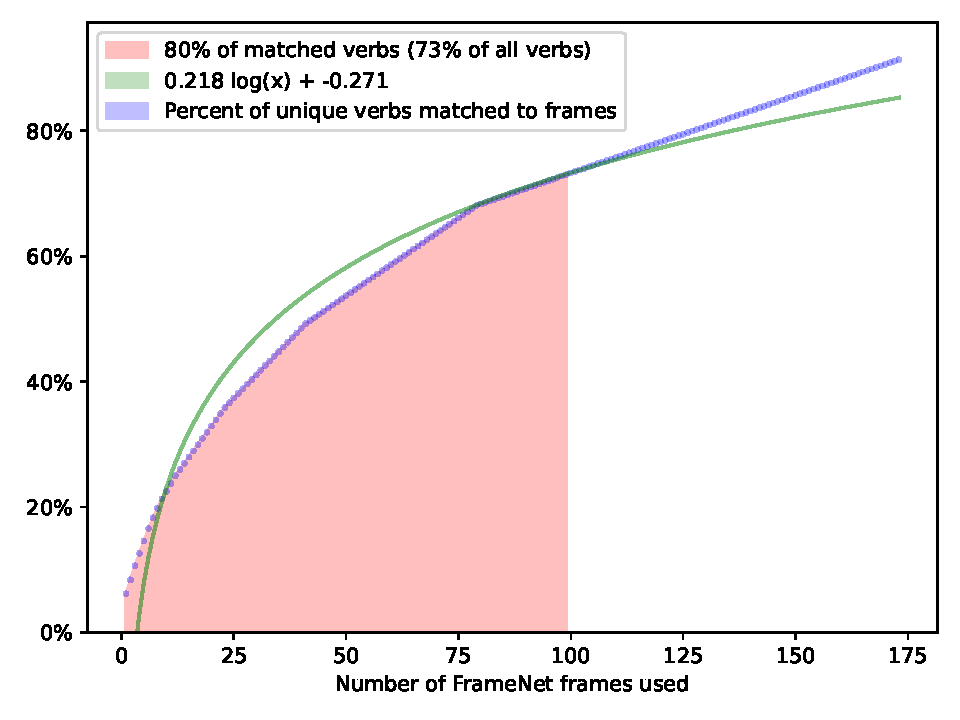
\includegraphics[width=0.75\columnwidth]{CH3_schemas/framenet_coverage}
    \caption{The results of an investigation into the number of verbs in a corpus that can be matched to FrameNet frames. A total of 91\% of verbs can be matched using automated FrameNet matching techniques. The region shaded in red shows that 80\% of all matched verbs can be covered by only 57\% of the total frames invoked across the corpus. The best-fit logarithm is overlaid in green for reference.}
    \label{fig:fn_coverage}
\end{figure}

\section{Protoschema Matching as FrameNet Parsing}
\label{sec:lome}

\begin{figure*}
    \centering
    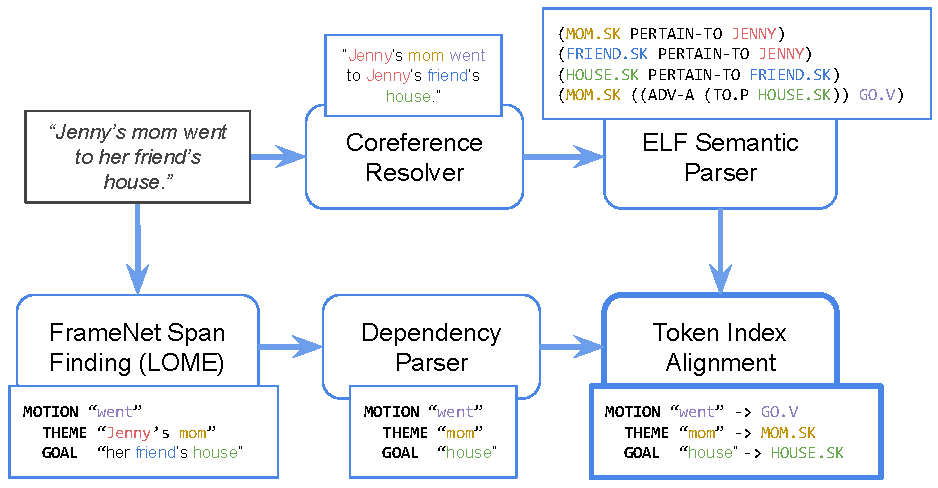
\includegraphics[width=\columnwidth]{figures/nesl/lome_architecture}
    \caption{A representation of the process by which FrameNet parsing with LOME is used for protoschema matching. The coreference resolver is provided by AllenNLP \citep{Gardner2017AllenNLP}, and the dependency parser is provided by spaCy \citep{spacy2}.}
    \label{fig:lome_architecture}
\end{figure*}

Our system's architecture, illustrated in Figure~\ref{fig:lome_architecture}, is divided into two main information pipelines: the EL track, responsible for semantic parsing, and the FrameNet track, responsible for frame identification and span selection. The information from both of these pipelines is unified into a final schematic representation at the end using token indices from the input text.

\subsection{EL Track}
To produce an EL semantic parse of the story, we first perform span mapping on the input text using the AllenNLP coreference resolver \citep{Gardner2017AllenNLP}. Co-referring token indices are saved, and story sentences are then converted into ELFs by first parsing them into ULF---an underspecified variant of EL \citep{kim2019IWCS}---and then processing the ULFs into full ELFs by converting grammatical tense information into temporal relations and scoping quantifiers. More information on the ELF parser can be found in \citep{Lawley2021LearningGE}.

Coreference resolution on the ELFs is performed by cross-referencing the token index clusters with token index tags placed on individuals in the EL parse. Co-referring individuals in the EL parse are then combined into one individual and substitutions are made throughout the parse.

\subsection{FrameNet Track}
To identify basic behavioral frames invoked by the raw text, we make use of the LOME information extraction system \citep{lome}. LOME outputs invoked frames, and text spans that fill frame roles, as \textsc{Concrete} data files. Once we extract the invoked frames and text spans, we perform a syntactic dependency parse on the input text using spaCy \citep{spacy2} and identify the first token in each span with a \texttt{NSUBJ}, \texttt{DOBJ}, or \texttt{POBJ} tag. This allows any span of text containing tokens for multiple individuals, e.g. \textit{her friend's house}, to be reduced to, e.g., \textit{house}, which will be the token used to identify the logical individual in the EL parse during the alignment phase.

\subsection{Token Index Alignment and Schema Formation}
To represent the identified FrameNet frames as EL formulas, the text spans that fill the semantic roles for each frame must first be bound to logical individuals. After the dependency parser identifies the token to cross-reference with the EL parse, the noun predicate with the same token index is retrieved from the EL parse, and the individual satisfying that predicate is identified as the bound value for the frame role.

The verb that invoked the frame is identified in a similar fashion, and a schema is created with that verb's formula from the EL parse as its header, and with the names of the FrameNet semantic roles applied to the relevant individuals as semantic types in the new schema's \texttt{Roles} section. When multiple frames are converted to schemas in this way, they may all be embedded together in a \textit{composite schema}, such as the one shown in Figure~\ref{fig:schema}, with their header formulas as steps and with each of their inner type constraints shown in the composite schema's \texttt{Roles} section for clarity. This composite schema forms our final semantic representation of the story.

%\section{Discussion}
%The goal of our representation, and of semantic story representations in general, is to enable a variety of reasoning tasks. We discuss two interesting potential applications of this representation here: question answering and event schema acquisition.